\section{Robust variable selection} 
The key problem that \citet{wang2013robust} try to investigate is the  characterization of robustness when combining a variable selection process to a robust regression problem. Mathematically, the regression problem is formulated as a  minimization of some penalized robust loss function, where the robustness comes from a proper choice of the loss function and the sparsity of the solution is encoded in the penalty term. In this section, we introduce the penalized robust regression objective function and set up the notation for this report.


\subsection{Exponential square loss function} \label{sec:esl}
In the setting of robust regression, we are given a set of data points $\{(x_i, y_i)_{i=1}^n: \forall i\in [d],  x_i \in \reals^d, y_i \in \reals\}$, where $x_i$ is referred as the covariates and $y_i$ is the response. Assuming that $(x_i, y_i)$ satisfying the linear regression model:
\[
y_i = x_i^T \beta +\eps_i, \quad \forall i = 1, 2, \dots , n,     
\] 
and the goal is to infer the coefficients $\beta \in \reals^d$. 

The authors consider the exponential square loss (ESL) function with a tuning parameter $\gamma$, i.e., $\phi_\gamma(t)= 1-  \exp (-t^2/\gamma)$. And the unregularized empirical loss is given by
\[
 \ell_n^* = 1- \frac{1}{n}\sum_{i = 1}^ n \exp \left\{ -(y_i- x_i^T\beta)^2/\gamma\right\}  .    
\]
As illustrated in \cref{fig:esl}(Left), in contrast to the traditional OLS loss, the boundedness of this loss function limits the influence of outliers that generates huge residual error and controls the bias of the estimator. And the  
parameter $\gamma$ controls the level of the robustness by setting different ``truncation level'' to large residuals---as displayed in \cref{fig:esl}(Right), 
smaller $\gamma$ leads to a more robust estimator; on the other hand, it may increase the variance of the estimator as it focuses on data points that generate small residual errors.  

One may notice that ESL loss is not convex, meaning that solving the regression problem requires a careful choice of the initial value and optimization algorithm.
A comprehensive discussion of the optimization algorithm will be presented in \cref{sec:computation}.




\begin{figure}[H]
    \centering
    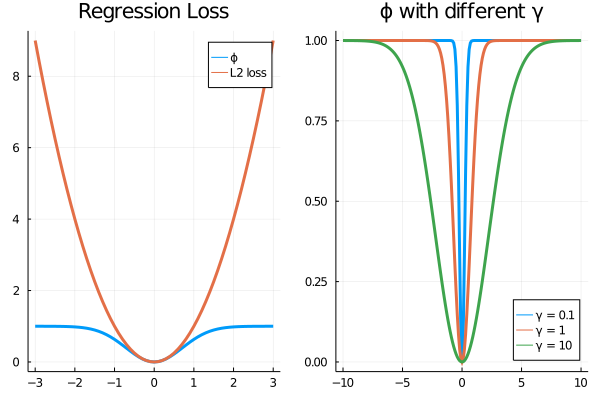
\includegraphics[width = 0.8\linewidth]{figures/esl.png}
    \caption{Figure of ESL loss function.}
    \label{fig:esl}
\end{figure}






\subsection{Regularizer} \label{sec:pnty}
Next, we introduce the regularization term that encodes the sparsity to the estimator, namely enables a variable selection. A typical choice is the $\ell_1$ penalization, i.e., $\|\beta\|_1$, which is widely used in a linear regression setting (LASSO). However, researchers find that the LASSO is not consistent in general, meaning that it may not recover the true underlying model asymptotically \citep{zhao2006model}. Therefore, \citet{wang2013robust} propose using the adaptive LASSO penalty \citep{zou2006adaptive} with tuning parameters $\tau_{nj}$, 
\[
p_{\tau}(\beta) = \sum_{j=1}^d \tau_{nj}|\beta_j|/|\tilde{\beta_j}|,   
\]
which can be viewed as a weighted version of $\ell_1$ norm.
Here $\tilde{\beta}$ is an pilot robust regression estimator, e.g., MM-estimator, S-estimator, OLS estimator, which should be chosen as a $\sqrt{n}$-consistent estimator. As suggested by the authors, we set $\tilde \beta$ as the MM-estimator, which later is also used as the initial value of the optimization algorithm. 


Intuitively, the regularizing constant $\tau \defined (\tau_{n1}, \dots, \tau_{nd}) $ controls the level of this weighted $\ell_1$ penalization, i.e., $\sum_{j = 1}^d \frac{\tau_{nj}}{|\tilde{\beta_j}|} |\beta_j|$. For a fixed pilot estimator $\tilde{\beta}$, larger value of $\tau$ tends to return a sparser estimator.  
The author suggest simply setting 
\[
 \tau_{n1} = \dots = \tau_{nd} = \frac{\log n}{n} =: \tau_n,
\] 
which comes from the minimization of a BIC-type objective function. Therefore, the ESL-LASSO estimator is defined as the minimizer of the following objective function:
\[\label{eq:esl_lasso}
\ell_n(\beta)  =    1- \frac{1}{n}\sum_{i = 1}^ n \exp \left\{ -(y_i- x_i^T\beta)^2/\gamma\right\} +  \tau_{n} \sum_{j=1}^d|\beta_j|/|\tilde{\beta_j}|.
\]
The goal of using this combination of $\tau_n$ and the adaptive LASSO penalty is to ensure a stronger asymptotic property for the ESL-LASSO estimator in terms of the variable selection process, which is called the \emph{oracle property} \citep{fan2001variable}---not only identifies the true coefficients in data asymptotic regime, but also obtains the optimal convergence rate. 






















